\documentclass[1p]{elsarticle_modified}
%\bibliographystyle{elsarticle-num}

%\usepackage[colorlinks]{hyperref}
%\usepackage{abbrmath_seonhwa} %\Abb, \Ascr, \Acal ,\Abf, \Afrak
\usepackage{amsfonts}
\usepackage{amssymb}
\usepackage{amsmath}
\usepackage{amsthm}
\usepackage{scalefnt}
\usepackage{amsbsy}
\usepackage{kotex}
\usepackage{caption}
\usepackage{subfig}
\usepackage{color}
\usepackage{graphicx}
\usepackage{xcolor} %% white, black, red, green, blue, cyan, magenta, yellow
\usepackage{float}
\usepackage{setspace}
\usepackage{hyperref}

\usepackage{tikz}
\usetikzlibrary{arrows}

\usepackage{multirow}
\usepackage{array} % fixed length table
\usepackage{hhline}

%%%%%%%%%%%%%%%%%%%%%
\makeatletter
\renewcommand*\env@matrix[1][\arraystretch]{%
	\edef\arraystretch{#1}%
	\hskip -\arraycolsep
	\let\@ifnextchar\new@ifnextchar
	\array{*\c@MaxMatrixCols c}}
\makeatother %https://tex.stackexchange.com/questions/14071/how-can-i-increase-the-line-spacing-in-a-matrix
%%%%%%%%%%%%%%%

\usepackage[normalem]{ulem}

\newcommand{\msout}[1]{\ifmmode\text{\sout{\ensuremath{#1}}}\else\sout{#1}\fi}
%SOURCE: \msout is \stkout macro in https://tex.stackexchange.com/questions/20609/strikeout-in-math-mode

\newcommand{\cancel}[1]{
	\ifmmode
	{\color{red}\msout{#1}}
	\else
	{\color{red}\sout{#1}}
	\fi
}

\newcommand{\add}[1]{
	{\color{blue}\uwave{#1}}
}

\newcommand{\replace}[2]{
	\ifmmode
	{\color{red}\msout{#1}}{\color{blue}\uwave{#2}}
	\else
	{\color{red}\sout{#1}}{\color{blue}\uwave{#2}}
	\fi
}

\newcommand{\Sol}{\mathcal{S}} %segment
\newcommand{\D}{D} %diagram
\newcommand{\A}{\mathcal{A}} %arc


%%%%%%%%%%%%%%%%%%%%%%%%%%%%%5 test

\def\sl{\operatorname{\textup{SL}}(2,\Cbb)}
\def\psl{\operatorname{\textup{PSL}}(2,\Cbb)}
\def\quan{\mkern 1mu \triangleright \mkern 1mu}

\theoremstyle{definition}
\newtheorem{thm}{Theorem}[section]
\newtheorem{prop}[thm]{Proposition}
\newtheorem{lem}[thm]{Lemma}
\newtheorem{ques}[thm]{Question}
\newtheorem{cor}[thm]{Corollary}
\newtheorem{defn}[thm]{Definition}
\newtheorem{exam}[thm]{Example}
\newtheorem{rmk}[thm]{Remark}
\newtheorem{alg}[thm]{Algorithm}

\newcommand{\I}{\sqrt{-1}}
\begin{document}

%\begin{frontmatter}
%
%\title{Boundary parabolic representations of knots up to 8 crossings}
%
%%% Group authors per affiliation:
%\author{Yunhi Cho} 
%\address{Department of Mathematics, University of Seoul, Seoul, Korea}
%\ead{yhcho@uos.ac.kr}
%
%
%\author{Seonhwa Kim} %\fnref{s_kim}}
%\address{Center for Geometry and Physics, Institute for Basic Science, Pohang, 37673, Korea}
%\ead{ryeona17@ibs.re.kr}
%
%\author{Hyuk Kim}
%\address{Department of Mathematical Sciences, Seoul National University, Seoul 08826, Korea}
%\ead{hyukkim@snu.ac.kr}
%
%\author{Seokbeom Yoon}
%\address{Department of Mathematical Sciences, Seoul National University, Seoul, 08826,  Korea}
%\ead{sbyoon15@snu.ac.kr}
%
%\begin{abstract}
%We find all boundary parabolic representation of knots up to 8 crossings.
%
%\end{abstract}
%\begin{keyword}
%    \MSC[2010] 57M25 
%\end{keyword}
%
%\end{frontmatter}

%\linenumbers
%\tableofcontents
%
\newcommand\colored[1]{\textcolor{white}{\rule[-0.35ex]{0.8em}{1.4ex}}\kern-0.8em\color{red} #1}%
%\newcommand\colored[1]{\textcolor{white}{ #1}\kern-2.17ex	\textcolor{white}{ #1}\kern-1.81ex	\textcolor{white}{ #1}\kern-2.15ex\color{red}#1	}

{\Large $\underline{12a_{0811}~(K12a_{0811})}$}

\setlength{\tabcolsep}{10pt}
\renewcommand{\arraystretch}{1.6}
\vspace{1cm}\begin{tabular}{m{100pt}>{\centering\arraybackslash}m{274pt}}
\multirow{5}{120pt}{
	\centering
	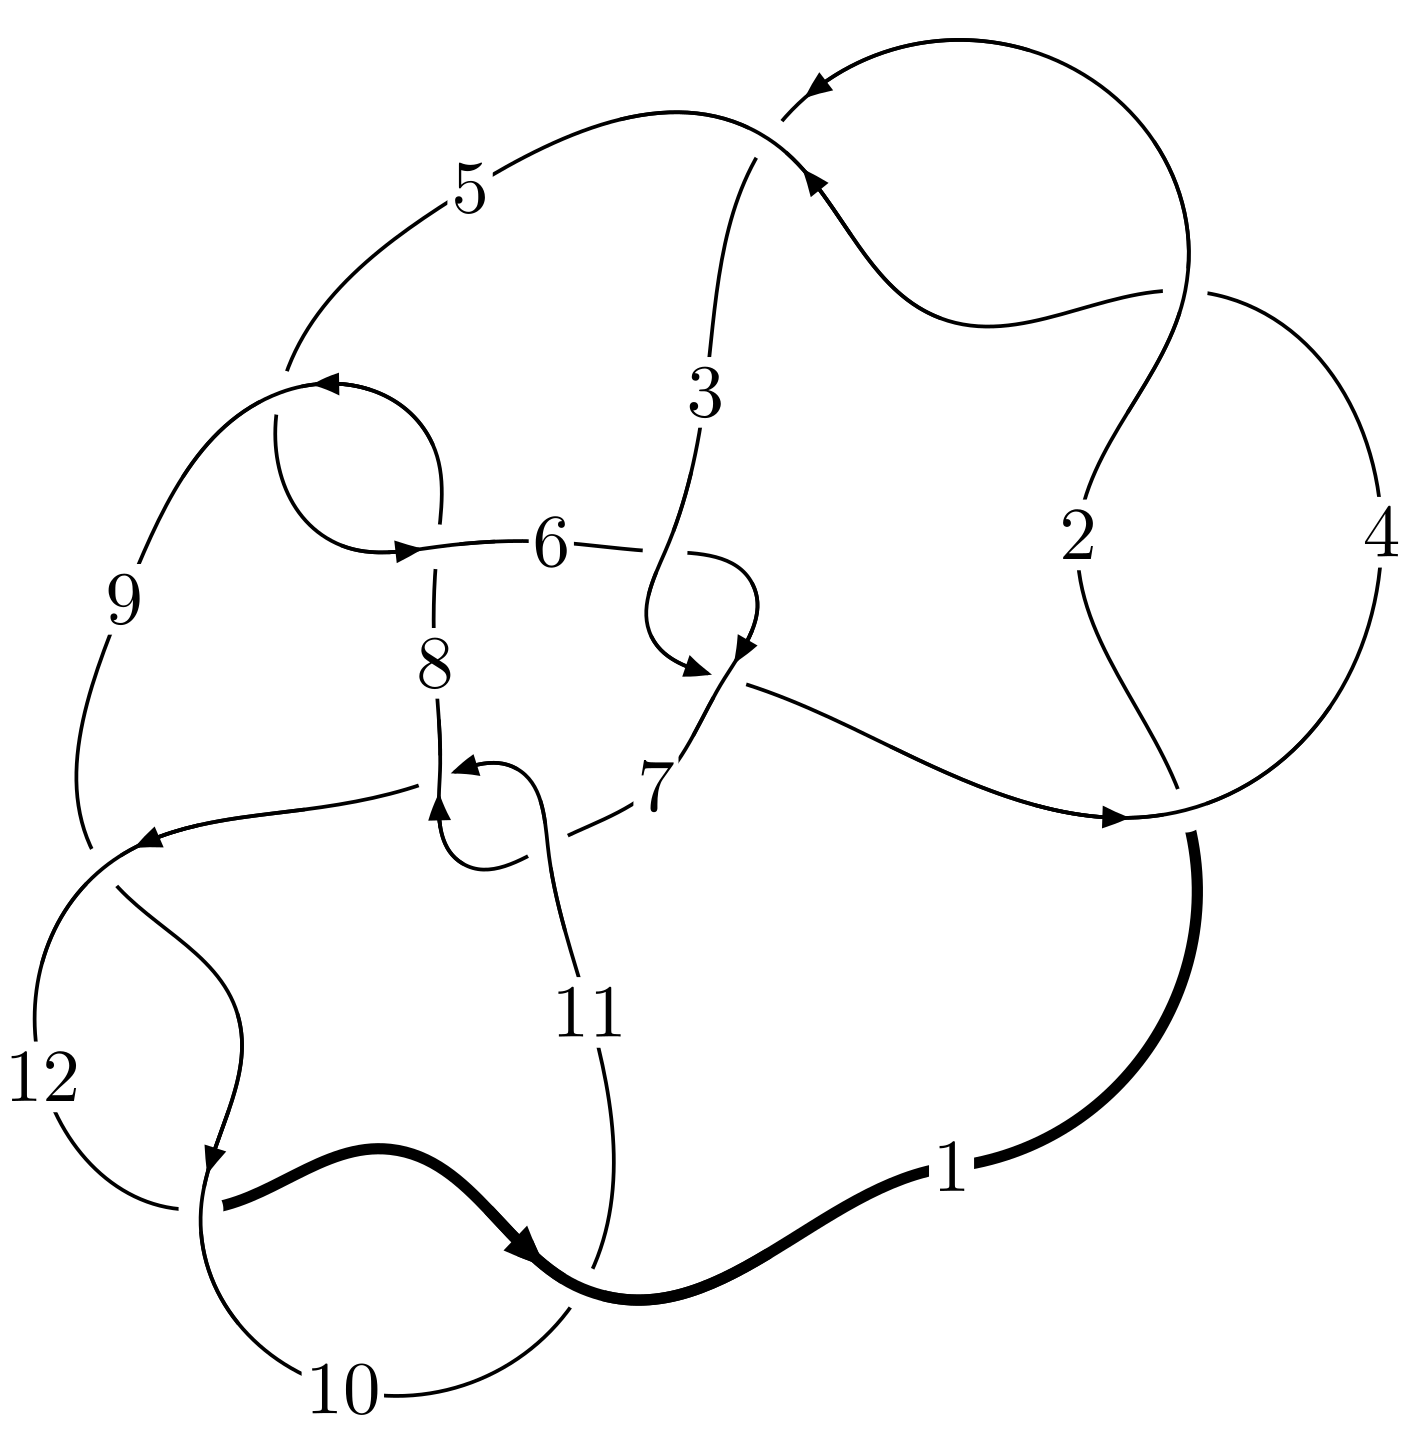
\includegraphics[width=112pt]{../../../GIT/diagram.site/Diagrams/png/1612_12a_0811.png}\\
\ \ \ A knot diagram\footnotemark}&
\allowdisplaybreaks
\textbf{Linearized knot diagam} \\
\cline{2-2}
 &
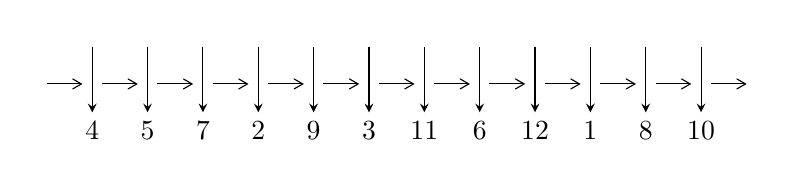
\begin{tikzpicture}[x=20pt, y=17pt]
	% nodes
	\node (C0) at (0, 0) {};
	\node (C1) at (1, 0) {};
	\node (C1U) at (1, +1) {};
	\node (C1D) at (1, -1) {4};

	\node (C2) at (2, 0) {};
	\node (C2U) at (2, +1) {};
	\node (C2D) at (2, -1) {5};

	\node (C3) at (3, 0) {};
	\node (C3U) at (3, +1) {};
	\node (C3D) at (3, -1) {7};

	\node (C4) at (4, 0) {};
	\node (C4U) at (4, +1) {};
	\node (C4D) at (4, -1) {2};

	\node (C5) at (5, 0) {};
	\node (C5U) at (5, +1) {};
	\node (C5D) at (5, -1) {9};

	\node (C6) at (6, 0) {};
	\node (C6U) at (6, +1) {};
	\node (C6D) at (6, -1) {3};

	\node (C7) at (7, 0) {};
	\node (C7U) at (7, +1) {};
	\node (C7D) at (7, -1) {11};

	\node (C8) at (8, 0) {};
	\node (C8U) at (8, +1) {};
	\node (C8D) at (8, -1) {6};

	\node (C9) at (9, 0) {};
	\node (C9U) at (9, +1) {};
	\node (C9D) at (9, -1) {12};

	\node (C10) at (10, 0) {};
	\node (C10U) at (10, +1) {};
	\node (C10D) at (10, -1) {1};

	\node (C11) at (11, 0) {};
	\node (C11U) at (11, +1) {};
	\node (C11D) at (11, -1) {8};

	\node (C12) at (12, 0) {};
	\node (C12U) at (12, +1) {};
	\node (C12D) at (12, -1) {10};
	\node (C13) at (13, 0) {};

	% arrows
	\draw[->,>={angle 60}]
	(C0) edge (C1) (C1) edge (C2) (C2) edge (C3) (C3) edge (C4) (C4) edge (C5) (C5) edge (C6) (C6) edge (C7) (C7) edge (C8) (C8) edge (C9) (C9) edge (C10) (C10) edge (C11) (C11) edge (C12) (C12) edge (C13) ;	\draw[->,>=stealth]
	(C1U) edge (C1D) (C2U) edge (C2D) (C3U) edge (C3D) (C4U) edge (C4D) (C5U) edge (C5D) (C6U) edge (C6D) (C7U) edge (C7D) (C8U) edge (C8D) (C9U) edge (C9D) (C10U) edge (C10D) (C11U) edge (C11D) (C12U) edge (C12D) ;
	\end{tikzpicture} \\
\hhline{~~} \\& 
\textbf{Solving Sequence} \\ \cline{2-2} 
 &
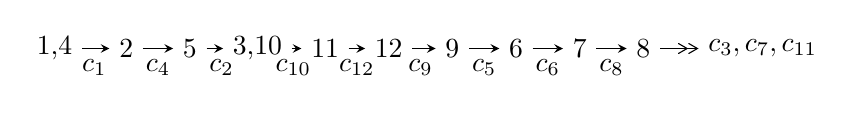
\begin{tikzpicture}[x=23pt, y=7pt]
	% node
	\node (A0) at (-1/8, 0) {1,4};
	\node (A1) at (1, 0) {2};
	\node (A2) at (2, 0) {5};
	\node (A3) at (49/16, 0) {3,10};
	\node (A4) at (33/8, 0) {11};
	\node (A5) at (41/8, 0) {12};
	\node (A6) at (49/8, 0) {9};
	\node (A7) at (57/8, 0) {6};
	\node (A8) at (65/8, 0) {7};
	\node (A9) at (73/8, 0) {8};
	\node (C1) at (1/2, -1) {$c_{1}$};
	\node (C2) at (3/2, -1) {$c_{4}$};
	\node (C3) at (5/2, -1) {$c_{2}$};
	\node (C4) at (29/8, -1) {$c_{10}$};
	\node (C5) at (37/8, -1) {$c_{12}$};
	\node (C6) at (45/8, -1) {$c_{9}$};
	\node (C7) at (53/8, -1) {$c_{5}$};
	\node (C8) at (61/8, -1) {$c_{6}$};
	\node (C9) at (69/8, -1) {$c_{8}$};
	\node (A10) at (11, 0) {$c_{3},c_{7},c_{11}$};

	% edge
	\draw[->,>=stealth]	
	(A0) edge (A1) (A1) edge (A2) (A2) edge (A3) (A3) edge (A4) (A4) edge (A5) (A5) edge (A6) (A6) edge (A7) (A7) edge (A8) (A8) edge (A9) ;
	\draw[->>,>={angle 60}]	
	(A9) edge (A10);
\end{tikzpicture} \\ 

\end{tabular} \\

\footnotetext{
The image of knot diagram is generated by the software ``\textbf{Draw programme}" developed by Andrew Bartholomew(\url{http://www.layer8.co.uk/maths/draw/index.htm\#Running-draw}), where we modified some parts for our purpose(\url{https://github.com/CATsTAILs/LinksPainter}).
}\phantom \\ \newline 
\centering \textbf{Ideals for irreducible components\footnotemark of $X_{\text{par}}$} 
 
\begin{align*}
I^u_{1}&=\langle 
b+u,\;-2 u^{17}-7 u^{16}+\cdots+2 a-7,\;u^{18}+3 u^{17}+\cdots+5 u-1\rangle \\
I^u_{2}&=\langle 
5.65807\times10^{75} u^{73}+4.34249\times10^{76} u^{72}+\cdots+1.46489\times10^{74} b-4.16421\times10^{75},\\
\phantom{I^u_{2}}&\phantom{= \langle  }1.50543\times10^{75} u^{73}+1.12371\times10^{76} u^{72}+\cdots+1.46489\times10^{74} a-3.11479\times10^{75},\;u^{74}+9 u^{73}+\cdots+25 u-1\rangle \\
I^u_{3}&=\langle 
b+1,\;-4 u^7-6 u^6+9 u^5+12 u^4-6 u^3-2 u^2+a- u-8,\;u^8+u^7-3 u^6-2 u^5+3 u^4+2 u-1\rangle \\
I^u_{4}&=\langle 
-1146 a^7+3254 a^6+13110 a^5-27698 a^4-23575 a^3+74422 a^2+661 b-44359 a+6376,\\
\phantom{I^u_{4}}&\phantom{= \langle  }a^8-3 a^7-11 a^6+26 a^5+17 a^4-68 a^3+48 a^2-12 a+1,\;u-1\rangle \\
I^u_{5}&=\langle 
b+u,\;a-2,\;u^2+u-1\rangle \\
I^u_{6}&=\langle 
b- u-1,\;a+u+1,\;u^2+u-1\rangle \\
\\
\end{align*}
\raggedright * 6 irreducible components of $\dim_{\mathbb{C}}=0$, with total 112 representations.\\
\footnotetext{All coefficients of polynomials are rational numbers. But the coefficients are sometimes approximated in decimal forms when there is not enough margin.}
\newpage
\renewcommand{\arraystretch}{1}
\centering \section*{I. $I^u_{1}= \langle b+u,\;-2 u^{17}-7 u^{16}+\cdots+2 a-7,\;u^{18}+3 u^{17}+\cdots+5 u-1 \rangle$}
\flushleft \textbf{(i) Arc colorings}\\
\begin{tabular}{m{7pt} m{180pt} m{7pt} m{180pt} }
\flushright $a_{1}=$&$\begin{pmatrix}1\\0\end{pmatrix}$ \\
\flushright $a_{4}=$&$\begin{pmatrix}0\\u\end{pmatrix}$ \\
\flushright $a_{2}=$&$\begin{pmatrix}1\\u^2\end{pmatrix}$ \\
\flushright $a_{5}=$&$\begin{pmatrix}- u\\- u^3+u\end{pmatrix}$ \\
\flushright $a_{3}=$&$\begin{pmatrix}- u^2+1\\- u^4+2 u^2\end{pmatrix}$ \\
\flushright $a_{10}=$&$\begin{pmatrix}u^{17}+\frac{7}{2} u^{16}+\cdots-2 u+\frac{7}{2}\\- u\end{pmatrix}$ \\
\flushright $a_{11}=$&$\begin{pmatrix}u^{17}+\frac{7}{2} u^{16}+\cdots- u+\frac{7}{2}\\- u\end{pmatrix}$ \\
\flushright $a_{12}=$&$\begin{pmatrix}\frac{1}{2} u^{17}+2 u^{16}+\cdots-\frac{3}{2} u+2\\- u^2\end{pmatrix}$ \\
\flushright $a_{9}=$&$\begin{pmatrix}\frac{1}{2} u^{17}+2 u^{16}+\cdots-\frac{3}{2} u+3\\u^3- u\end{pmatrix}$ \\
\flushright $a_{6}=$&$\begin{pmatrix}\frac{1}{2} u^{17}-\frac{9}{2} u^{15}+\cdots+\frac{5}{2} u-2\\-\frac{1}{2} u^{17}-\frac{1}{2} u^{16}+\cdots-\frac{3}{2} u+\frac{1}{2}\end{pmatrix}$ \\
\flushright $a_{7}=$&$\begin{pmatrix}-\frac{1}{2} u^{16}- u^{15}+\cdots+3 u-\frac{5}{2}\\-2 u^{17}-3 u^{16}+\cdots-10 u+2\end{pmatrix}$ \\
\flushright $a_{8}=$&$\begin{pmatrix}u^{17}+3 u^{16}+\cdots-3 u+4\\\frac{5}{2} u^{17}+\frac{9}{2} u^{16}+\cdots+\frac{25}{2} u-\frac{5}{2}\end{pmatrix}$\\&\end{tabular}
\flushleft \textbf{(ii) Obstruction class $= -1$}\\~\\
\flushleft \textbf{(iii) Cusp Shapes $= 3 u^{17}+4 u^{16}-25 u^{15}-30 u^{14}+79 u^{13}+59 u^{12}-138 u^{11}+24 u^{10}+161 u^9-176 u^8-68 u^7+150 u^6-100 u^5-11 u^4+62 u^3-42 u^2+33 u-16$}\\~\\
\newpage\renewcommand{\arraystretch}{1}
\flushleft \textbf{(iv) u-Polynomials at the component}\newline \\
\begin{tabular}{m{50pt}|m{274pt}}
Crossings & \hspace{64pt}u-Polynomials at each crossing \\
\hline $$\begin{aligned}c_{1},c_{2},c_{4}\\c_{9},c_{10},c_{12}\end{aligned}$$&$\begin{aligned}
&u^{18}-3 u^{17}+\cdots-5 u-1
\end{aligned}$\\
\hline $$\begin{aligned}c_{3},c_{6},c_{7}\\c_{11}\end{aligned}$$&$\begin{aligned}
&u^{18}+u^{17}+\cdots-5 u-1
\end{aligned}$\\
\hline $$\begin{aligned}c_{5},c_{8}\end{aligned}$$&$\begin{aligned}
&u^{18}-5 u^{17}+\cdots-8 u+4
\end{aligned}$\\
\hline
\end{tabular}\\~\\
\newpage\renewcommand{\arraystretch}{1}
\flushleft \textbf{(v) Riley Polynomials at the component}\newline \\
\begin{tabular}{m{50pt}|m{274pt}}
Crossings & \hspace{64pt}Riley Polynomials at each crossing \\
\hline $$\begin{aligned}c_{1},c_{2},c_{4}\\c_{9},c_{10},c_{12}\end{aligned}$$&$\begin{aligned}
&y^{18}-17 y^{17}+\cdots-19 y+1
\end{aligned}$\\
\hline $$\begin{aligned}c_{3},c_{6},c_{7}\\c_{11}\end{aligned}$$&$\begin{aligned}
&y^{18}-9 y^{17}+\cdots-11 y+1
\end{aligned}$\\
\hline $$\begin{aligned}c_{5},c_{8}\end{aligned}$$&$\begin{aligned}
&y^{18}+5 y^{17}+\cdots+96 y+16
\end{aligned}$\\
\hline
\end{tabular}\\~\\
\newpage\flushleft \textbf{(vi) Complex Volumes and Cusp Shapes}
$$\begin{array}{c|c|c}  
\text{Solutions to }I^u_{1}& \I (\text{vol} + \sqrt{-1}CS) & \text{Cusp shape}\\
 \hline 
\begin{aligned}
u &= \phantom{-}0.989632 + 0.118366 I \\
a &= -4.73699 + 1.01751 I \\
b &= -0.989632 - 0.118366 I\end{aligned}
 & -2.95901 - 0.54782 I & -26.1989 - 20.7388 I \\ \hline\begin{aligned}
u &= \phantom{-}0.989632 - 0.118366 I \\
a &= -4.73699 - 1.01751 I \\
b &= -0.989632 + 0.118366 I\end{aligned}
 & -2.95901 + 0.54782 I & -26.1989 + 20.7388 I \\ \hline\begin{aligned}
u &= \phantom{-}0.422326 + 0.866115 I \\
a &= -0.292665 + 0.821087 I \\
b &= -0.422326 - 0.866115 I\end{aligned}
 & -1.45893 - 7.65022 I & -14.1263 + 7.9961 I \\ \hline\begin{aligned}
u &= \phantom{-}0.422326 - 0.866115 I \\
a &= -0.292665 - 0.821087 I \\
b &= -0.422326 + 0.866115 I\end{aligned}
 & -1.45893 + 7.65022 I & -14.1263 - 7.9961 I \\ \hline\begin{aligned}
u &= \phantom{-}0.505624 + 0.659339 I \\
a &= -0.37939 + 1.54732 I \\
b &= -0.505624 - 0.659339 I\end{aligned}
 & -2.76095 - 2.16079 I & -16.8057 + 4.7341 I \\ \hline\begin{aligned}
u &= \phantom{-}0.505624 - 0.659339 I \\
a &= -0.37939 - 1.54732 I \\
b &= -0.505624 + 0.659339 I\end{aligned}
 & -2.76095 + 2.16079 I & -16.8057 - 4.7341 I \\ \hline\begin{aligned}
u &= -1.217590 + 0.250614 I \\
a &= \phantom{-}0.999646 + 0.475841 I \\
b &= \phantom{-}1.217590 - 0.250614 I\end{aligned}
 & -4.05098 + 7.39685 I & -19.0054 - 11.1633 I \\ \hline\begin{aligned}
u &= -1.217590 - 0.250614 I \\
a &= \phantom{-}0.999646 - 0.475841 I \\
b &= \phantom{-}1.217590 + 0.250614 I\end{aligned}
 & -4.05098 - 7.39685 I & -19.0054 + 11.1633 I \\ \hline\begin{aligned}
u &= -1.24743\phantom{ +0.000000I} \\
a &= \phantom{-}0.531653\phantom{ +0.000000I} \\
b &= \phantom{-}1.24743\phantom{ +0.000000I}\end{aligned}
 & -9.19331\phantom{ +0.000000I} & -28.9570\phantom{ +0.000000I} \\ \hline\begin{aligned}
u &= \phantom{-}1.41940 + 0.07138 I \\
a &= -3.39301 + 0.09249 I \\
b &= -1.41940 - 0.07138 I\end{aligned}
 & -6.53479 - 2.67378 I & -17.5529 + 2.6003 I\\
 \hline 
 \end{array}$$\newpage$$\begin{array}{c|c|c}  
\text{Solutions to }I^u_{1}& \I (\text{vol} + \sqrt{-1}CS) & \text{Cusp shape}\\
 \hline 
\begin{aligned}
u &= \phantom{-}1.41940 - 0.07138 I \\
a &= -3.39301 - 0.09249 I \\
b &= -1.41940 + 0.07138 I\end{aligned}
 & -6.53479 + 2.67378 I & -17.5529 - 2.6003 I \\ \hline\begin{aligned}
u &= -0.072733 + 0.557292 I \\
a &= \phantom{-}1.025250 + 0.580717 I \\
b &= \phantom{-}0.072733 - 0.557292 I\end{aligned}
 & \phantom{-}2.91333 - 1.30971 I & -5.30920 + 2.88857 I \\ \hline\begin{aligned}
u &= -0.072733 - 0.557292 I \\
a &= \phantom{-}1.025250 - 0.580717 I \\
b &= \phantom{-}0.072733 + 0.557292 I\end{aligned}
 & \phantom{-}2.91333 + 1.30971 I & -5.30920 - 2.88857 I \\ \hline\begin{aligned}
u &= -1.49614 + 0.31846 I \\
a &= \phantom{-}1.58598 + 1.29639 I \\
b &= \phantom{-}1.49614 - 0.31846 I\end{aligned}
 & -15.4055 + 9.6614 I & -20.3543 - 4.9770 I \\ \hline\begin{aligned}
u &= -1.49614 - 0.31846 I \\
a &= \phantom{-}1.58598 - 1.29639 I \\
b &= \phantom{-}1.49614 + 0.31846 I\end{aligned}
 & -15.4055 - 9.6614 I & -20.3543 + 4.9770 I \\ \hline\begin{aligned}
u &= -1.53609 + 0.37024 I \\
a &= \phantom{-}1.87364 + 1.16526 I \\
b &= \phantom{-}1.53609 - 0.37024 I\end{aligned}
 & -14.0740 + 16.8703 I & -19.0655 - 8.3694 I \\ \hline\begin{aligned}
u &= -1.53609 - 0.37024 I \\
a &= \phantom{-}1.87364 - 1.16526 I \\
b &= \phantom{-}1.53609 + 0.37024 I\end{aligned}
 & -14.0740 - 16.8703 I & -19.0655 + 8.3694 I \\ \hline\begin{aligned}
u &= \phantom{-}0.218580\phantom{ +0.000000I} \\
a &= \phantom{-}3.10342\phantom{ +0.000000I} \\
b &= -0.218580\phantom{ +0.000000I}\end{aligned}
 & -0.840991\phantom{ +0.000000I} & -10.2070\phantom{ +0.000000I}\\
 \hline 
 \end{array}$$\newpage\newpage\renewcommand{\arraystretch}{1}
\centering \section*{II. $I^u_{2}= \langle 5.66\times10^{75} u^{73}+4.34\times10^{76} u^{72}+\cdots+1.46\times10^{74} b-4.16\times10^{75},\;1.51\times10^{75} u^{73}+1.12\times10^{76} u^{72}+\cdots+1.46\times10^{74} a-3.11\times10^{75},\;u^{74}+9 u^{73}+\cdots+25 u-1 \rangle$}
\flushleft \textbf{(i) Arc colorings}\\
\begin{tabular}{m{7pt} m{180pt} m{7pt} m{180pt} }
\flushright $a_{1}=$&$\begin{pmatrix}1\\0\end{pmatrix}$ \\
\flushright $a_{4}=$&$\begin{pmatrix}0\\u\end{pmatrix}$ \\
\flushright $a_{2}=$&$\begin{pmatrix}1\\u^2\end{pmatrix}$ \\
\flushright $a_{5}=$&$\begin{pmatrix}- u\\- u^3+u\end{pmatrix}$ \\
\flushright $a_{3}=$&$\begin{pmatrix}- u^2+1\\- u^4+2 u^2\end{pmatrix}$ \\
\flushright $a_{10}=$&$\begin{pmatrix}-10.2768 u^{73}-76.7095 u^{72}+\cdots-183.962 u+21.2630\\-38.6246 u^{73}-296.439 u^{72}+\cdots-742.347 u+28.4268\end{pmatrix}$ \\
\flushright $a_{11}=$&$\begin{pmatrix}28.3478 u^{73}+219.729 u^{72}+\cdots+558.384 u-7.16380\\-38.6246 u^{73}-296.439 u^{72}+\cdots-742.347 u+28.4268\end{pmatrix}$ \\
\flushright $a_{12}=$&$\begin{pmatrix}-55.0611 u^{73}-413.482 u^{72}+\cdots-963.034 u+44.1715\\-100.725 u^{73}-764.026 u^{72}+\cdots-1830.80 u+71.0456\end{pmatrix}$ \\
\flushright $a_{9}=$&$\begin{pmatrix}33.4992 u^{73}+261.898 u^{72}+\cdots+709.028 u-16.0765\\75.6177 u^{73}+583.270 u^{72}+\cdots+1498.50 u-58.5028\end{pmatrix}$ \\
\flushright $a_{6}=$&$\begin{pmatrix}-30.8792 u^{73}-233.688 u^{72}+\cdots-554.094 u+16.6614\\-48.3000 u^{73}-364.699 u^{72}+\cdots-849.392 u+33.2488\end{pmatrix}$ \\
\flushright $a_{7}=$&$\begin{pmatrix}36.0803 u^{73}+270.250 u^{72}+\cdots+606.729 u-28.7422\\-25.1044 u^{73}-186.311 u^{72}+\cdots-406.556 u+16.0348\end{pmatrix}$ \\
\flushright $a_{8}=$&$\begin{pmatrix}32.0304 u^{73}+249.765 u^{72}+\cdots+672.873 u-12.6030\\13.2898 u^{73}+102.925 u^{72}+\cdots+269.186 u-10.8565\end{pmatrix}$\\&\end{tabular}
\flushleft \textbf{(ii) Obstruction class $= -1$}\\~\\
\flushleft \textbf{(iii) Cusp Shapes $= -18.3007 u^{73}-137.274 u^{72}+\cdots-108.453 u-7.83721$}\\~\\
\newpage\renewcommand{\arraystretch}{1}
\flushleft \textbf{(iv) u-Polynomials at the component}\newline \\
\begin{tabular}{m{50pt}|m{274pt}}
Crossings & \hspace{64pt}u-Polynomials at each crossing \\
\hline $$\begin{aligned}c_{1},c_{2},c_{4}\\c_{9},c_{10},c_{12}\end{aligned}$$&$\begin{aligned}
&u^{74}-9 u^{73}+\cdots-25 u-1
\end{aligned}$\\
\hline $$\begin{aligned}c_{3},c_{6},c_{7}\\c_{11}\end{aligned}$$&$\begin{aligned}
&u^{74}+3 u^{73}+\cdots-384 u-256
\end{aligned}$\\
\hline $$\begin{aligned}c_{5},c_{8}\end{aligned}$$&$\begin{aligned}
&(u^{37}+u^{36}+\cdots-9 u+2)^{2}
\end{aligned}$\\
\hline
\end{tabular}\\~\\
\newpage\renewcommand{\arraystretch}{1}
\flushleft \textbf{(v) Riley Polynomials at the component}\newline \\
\begin{tabular}{m{50pt}|m{274pt}}
Crossings & \hspace{64pt}Riley Polynomials at each crossing \\
\hline $$\begin{aligned}c_{1},c_{2},c_{4}\\c_{9},c_{10},c_{12}\end{aligned}$$&$\begin{aligned}
&y^{74}-75 y^{73}+\cdots-675 y+1
\end{aligned}$\\
\hline $$\begin{aligned}c_{3},c_{6},c_{7}\\c_{11}\end{aligned}$$&$\begin{aligned}
&y^{74}-51 y^{73}+\cdots-5160960 y+65536
\end{aligned}$\\
\hline $$\begin{aligned}c_{5},c_{8}\end{aligned}$$&$\begin{aligned}
&(y^{37}+15 y^{36}+\cdots+89 y-4)^{2}
\end{aligned}$\\
\hline
\end{tabular}\\~\\
\newpage\flushleft \textbf{(vi) Complex Volumes and Cusp Shapes}
$$\begin{array}{c|c|c}  
\text{Solutions to }I^u_{2}& \I (\text{vol} + \sqrt{-1}CS) & \text{Cusp shape}\\
 \hline 
\begin{aligned}
u &= \phantom{-}0.987559\phantom{ +0.000000I} \\
a &= \phantom{-}6.51633\phantom{ +0.000000I} \\
b &= -0.530694\phantom{ +0.000000I}\end{aligned}
 & -2.53018\phantom{ +0.000000I} & \phantom{-0.000000 } 0 \\ \hline\begin{aligned}
u &= \phantom{-}0.765958 + 0.687849 I \\
a &= \phantom{-}0.530736 - 0.170061 I \\
b &= -0.454310 + 0.712668 I\end{aligned}
 & -2.53529 + 2.33569 I & \phantom{-0.000000 } 0 \\ \hline\begin{aligned}
u &= \phantom{-}0.765958 - 0.687849 I \\
a &= \phantom{-}0.530736 + 0.170061 I \\
b &= -0.454310 - 0.712668 I\end{aligned}
 & -2.53529 - 2.33569 I & \phantom{-0.000000 } 0 \\ \hline\begin{aligned}
u &= \phantom{-}0.740221 + 0.600682 I \\
a &= \phantom{-}0.324726 - 0.192964 I \\
b &= \phantom{-}1.56736 - 0.14197 I\end{aligned}
 & -10.44390 + 0.43302 I & \phantom{-0.000000 } 0 \\ \hline\begin{aligned}
u &= \phantom{-}0.740221 - 0.600682 I \\
a &= \phantom{-}0.324726 + 0.192964 I \\
b &= \phantom{-}1.56736 + 0.14197 I\end{aligned}
 & -10.44390 - 0.43302 I & \phantom{-0.000000 } 0 \\ \hline\begin{aligned}
u &= \phantom{-}0.642782 + 0.680172 I \\
a &= -1.39299 + 1.23146 I \\
b &= -1.364200 + 0.024112 I\end{aligned}
 & -4.74326 + 0.09745 I & \phantom{-0.000000 } 0 \\ \hline\begin{aligned}
u &= \phantom{-}0.642782 - 0.680172 I \\
a &= -1.39299 - 1.23146 I \\
b &= -1.364200 - 0.024112 I\end{aligned}
 & -4.74326 - 0.09745 I & \phantom{-0.000000 } 0 \\ \hline\begin{aligned}
u &= \phantom{-}0.444752 + 0.973604 I \\
a &= \phantom{-}0.671707 - 1.134520 I \\
b &= \phantom{-}1.50776 + 0.32383 I\end{aligned}
 & -7.6984 - 11.9811 I & \phantom{-0.000000 } 0 \\ \hline\begin{aligned}
u &= \phantom{-}0.444752 - 0.973604 I \\
a &= \phantom{-}0.671707 + 1.134520 I \\
b &= \phantom{-}1.50776 - 0.32383 I\end{aligned}
 & -7.6984 + 11.9811 I & \phantom{-0.000000 } 0 \\ \hline\begin{aligned}
u &= \phantom{-}0.397060 + 0.840047 I \\
a &= \phantom{-}0.12647 - 1.41487 I \\
b &= \phantom{-}1.50364 + 0.23324 I\end{aligned}
 & -9.28734 - 5.43922 I & \phantom{-0.000000 } 0\\
 \hline 
 \end{array}$$\newpage$$\begin{array}{c|c|c}  
\text{Solutions to }I^u_{2}& \I (\text{vol} + \sqrt{-1}CS) & \text{Cusp shape}\\
 \hline 
\begin{aligned}
u &= \phantom{-}0.397060 - 0.840047 I \\
a &= \phantom{-}0.12647 + 1.41487 I \\
b &= \phantom{-}1.50364 - 0.23324 I\end{aligned}
 & -9.28734 + 5.43922 I & \phantom{-0.000000 } 0 \\ \hline\begin{aligned}
u &= \phantom{-}0.458933 + 0.804344 I \\
a &= -1.168670 + 0.748598 I \\
b &= -1.44440 - 0.12650 I\end{aligned}
 & -4.11115 - 5.12689 I & \phantom{-0.000000 } 0 \\ \hline\begin{aligned}
u &= \phantom{-}0.458933 - 0.804344 I \\
a &= -1.168670 - 0.748598 I \\
b &= -1.44440 + 0.12650 I\end{aligned}
 & -4.11115 + 5.12689 I & \phantom{-0.000000 } 0 \\ \hline\begin{aligned}
u &= \phantom{-}1.009020 + 0.377651 I \\
a &= \phantom{-}0.396161 - 0.004528 I \\
b &= \phantom{-}0.000170 - 0.316182 I\end{aligned}
 & -0.560067 - 0.765120 I & \phantom{-0.000000 } 0 \\ \hline\begin{aligned}
u &= \phantom{-}1.009020 - 0.377651 I \\
a &= \phantom{-}0.396161 + 0.004528 I \\
b &= \phantom{-}0.000170 + 0.316182 I\end{aligned}
 & -0.560067 + 0.765120 I & \phantom{-0.000000 } 0 \\ \hline\begin{aligned}
u &= -0.062358 + 0.874395 I \\
a &= -0.026642 + 0.252961 I \\
b &= \phantom{-}1.306060 + 0.081958 I\end{aligned}
 & -0.68340 - 3.31809 I & \phantom{-0.000000 } 0 \\ \hline\begin{aligned}
u &= -0.062358 - 0.874395 I \\
a &= -0.026642 - 0.252961 I \\
b &= \phantom{-}1.306060 - 0.081958 I\end{aligned}
 & -0.68340 + 3.31809 I & \phantom{-0.000000 } 0 \\ \hline\begin{aligned}
u &= \phantom{-}0.454310 + 0.712668 I \\
a &= \phantom{-}0.098685 - 0.671650 I \\
b &= -0.765958 + 0.687849 I\end{aligned}
 & -2.53529 - 2.33569 I & \phantom{-0.000000 } 0 \\ \hline\begin{aligned}
u &= \phantom{-}0.454310 - 0.712668 I \\
a &= \phantom{-}0.098685 + 0.671650 I \\
b &= -0.765958 - 0.687849 I\end{aligned}
 & -2.53529 + 2.33569 I & \phantom{-0.000000 } 0 \\ \hline\begin{aligned}
u &= \phantom{-}0.844818 + 0.836713 I \\
a &= \phantom{-}0.790427 - 0.298727 I \\
b &= \phantom{-}1.49740 - 0.26016 I\end{aligned}
 & -8.87079 + 5.90908 I & \phantom{-0.000000 } 0\\
 \hline 
 \end{array}$$\newpage$$\begin{array}{c|c|c}  
\text{Solutions to }I^u_{2}& \I (\text{vol} + \sqrt{-1}CS) & \text{Cusp shape}\\
 \hline 
\begin{aligned}
u &= \phantom{-}0.844818 - 0.836713 I \\
a &= \phantom{-}0.790427 + 0.298727 I \\
b &= \phantom{-}1.49740 + 0.26016 I\end{aligned}
 & -8.87079 - 5.90908 I & \phantom{-0.000000 } 0 \\ \hline\begin{aligned}
u &= \phantom{-}0.231667 + 0.747835 I \\
a &= \phantom{-}0.427670 - 0.319614 I \\
b &= \phantom{-}0.342720 + 0.342406 I\end{aligned}
 & \phantom{-}1.71361 - 3.34095 I & -7.14073 + 5.07807 I \\ \hline\begin{aligned}
u &= \phantom{-}0.231667 - 0.747835 I \\
a &= \phantom{-}0.427670 + 0.319614 I \\
b &= \phantom{-}0.342720 - 0.342406 I\end{aligned}
 & \phantom{-}1.71361 + 3.34095 I & -7.14073 - 5.07807 I \\ \hline\begin{aligned}
u &= \phantom{-}0.719088\phantom{ +0.000000I} \\
a &= -1.78155\phantom{ +0.000000I} \\
b &= \phantom{-}1.60418\phantom{ +0.000000I}\end{aligned}
 & -9.95403\phantom{ +0.000000I} & -72.0690\phantom{ +0.000000I} \\ \hline\begin{aligned}
u &= \phantom{-}1.265280 + 0.210357 I \\
a &= \phantom{-}1.098350 + 0.079438 I \\
b &= \phantom{-}0.218129 + 0.234231 I\end{aligned}
 & -1.19152 - 1.56254 I & \phantom{-0.000000 } 0 \\ \hline\begin{aligned}
u &= \phantom{-}1.265280 - 0.210357 I \\
a &= \phantom{-}1.098350 - 0.079438 I \\
b &= \phantom{-}0.218129 - 0.234231 I\end{aligned}
 & -1.19152 + 1.56254 I & \phantom{-0.000000 } 0 \\ \hline\begin{aligned}
u &= -1.306060 + 0.081958 I \\
a &= \phantom{-}0.169294 - 0.019291 I \\
b &= \phantom{-}0.062358 + 0.874395 I\end{aligned}
 & -0.68340 + 3.31809 I & \phantom{-0.000000 } 0 \\ \hline\begin{aligned}
u &= -1.306060 - 0.081958 I \\
a &= \phantom{-}0.169294 + 0.019291 I \\
b &= \phantom{-}0.062358 - 0.874395 I\end{aligned}
 & -0.68340 - 3.31809 I & \phantom{-0.000000 } 0 \\ \hline\begin{aligned}
u &= -0.595869 + 0.339811 I \\
a &= \phantom{-}1.72234 + 1.01149 I \\
b &= \phantom{-}1.38711 - 0.28497 I\end{aligned}
 & -3.44427 + 7.05663 I & -11.58513 - 7.17023 I \\ \hline\begin{aligned}
u &= -0.595869 - 0.339811 I \\
a &= \phantom{-}1.72234 - 1.01149 I \\
b &= \phantom{-}1.38711 + 0.28497 I\end{aligned}
 & -3.44427 - 7.05663 I & -11.58513 + 7.17023 I\\
 \hline 
 \end{array}$$\newpage$$\begin{array}{c|c|c}  
\text{Solutions to }I^u_{2}& \I (\text{vol} + \sqrt{-1}CS) & \text{Cusp shape}\\
 \hline 
\begin{aligned}
u &= \phantom{-}1.364200 + 0.024112 I \\
a &= -1.267920 + 0.136700 I \\
b &= -0.642782 + 0.680172 I\end{aligned}
 & -4.74326 - 0.09745 I & \phantom{-0.000000 } 0 \\ \hline\begin{aligned}
u &= \phantom{-}1.364200 - 0.024112 I \\
a &= -1.267920 - 0.136700 I \\
b &= -0.642782 - 0.680172 I\end{aligned}
 & -4.74326 + 0.09745 I & \phantom{-0.000000 } 0 \\ \hline\begin{aligned}
u &= -1.366460 + 0.029279 I \\
a &= -1.41815 - 0.40189 I \\
b &= -1.290050 + 0.520157 I\end{aligned}
 & -4.82697 + 1.65745 I & \phantom{-0.000000 } 0 \\ \hline\begin{aligned}
u &= -1.366460 - 0.029279 I \\
a &= -1.41815 + 0.40189 I \\
b &= -1.290050 - 0.520157 I\end{aligned}
 & -4.82697 - 1.65745 I & \phantom{-0.000000 } 0 \\ \hline\begin{aligned}
u &= \phantom{-}1.290050 + 0.520157 I \\
a &= \phantom{-}1.16345 - 0.86262 I \\
b &= \phantom{-}1.366460 + 0.029279 I\end{aligned}
 & -4.82697 - 1.65745 I & \phantom{-0.000000 } 0 \\ \hline\begin{aligned}
u &= \phantom{-}1.290050 - 0.520157 I \\
a &= \phantom{-}1.16345 + 0.86262 I \\
b &= \phantom{-}1.366460 - 0.029279 I\end{aligned}
 & -4.82697 + 1.65745 I & \phantom{-0.000000 } 0 \\ \hline\begin{aligned}
u &= \phantom{-}1.40953 + 0.12805 I \\
a &= \phantom{-}2.51596 - 1.15937 I \\
b &= \phantom{-}1.54388 + 0.20125 I\end{aligned}
 & -11.93780 - 3.04537 I & \phantom{-0.000000 } 0 \\ \hline\begin{aligned}
u &= \phantom{-}1.40953 - 0.12805 I \\
a &= \phantom{-}2.51596 + 1.15937 I \\
b &= \phantom{-}1.54388 - 0.20125 I\end{aligned}
 & -11.93780 + 3.04537 I & \phantom{-0.000000 } 0 \\ \hline\begin{aligned}
u &= -1.38711 + 0.28497 I \\
a &= \phantom{-}0.945189 + 0.206760 I \\
b &= \phantom{-}0.595869 - 0.339811 I\end{aligned}
 & -3.44427 + 7.05663 I & \phantom{-0.000000 } 0 \\ \hline\begin{aligned}
u &= -1.38711 - 0.28497 I \\
a &= \phantom{-}0.945189 - 0.206760 I \\
b &= \phantom{-}0.595869 + 0.339811 I\end{aligned}
 & -3.44427 - 7.05663 I & \phantom{-0.000000 } 0\\
 \hline 
 \end{array}$$\newpage$$\begin{array}{c|c|c}  
\text{Solutions to }I^u_{2}& \I (\text{vol} + \sqrt{-1}CS) & \text{Cusp shape}\\
 \hline 
\begin{aligned}
u &= -1.43299 + 0.09516 I \\
a &= \phantom{-}0.755112 + 0.316373 I \\
b &= \phantom{-}0.251570 - 0.421107 I\end{aligned}
 & -6.60087 + 1.06308 I & \phantom{-0.000000 } 0 \\ \hline\begin{aligned}
u &= -1.43299 - 0.09516 I \\
a &= \phantom{-}0.755112 - 0.316373 I \\
b &= \phantom{-}0.251570 + 0.421107 I\end{aligned}
 & -6.60087 - 1.06308 I & \phantom{-0.000000 } 0 \\ \hline\begin{aligned}
u &= \phantom{-}1.44440 + 0.12650 I \\
a &= -0.818084 - 0.341295 I \\
b &= -0.458933 - 0.804344 I\end{aligned}
 & -4.11115 - 5.12689 I & \phantom{-0.000000 } 0 \\ \hline\begin{aligned}
u &= \phantom{-}1.44440 - 0.12650 I \\
a &= -0.818084 + 0.341295 I \\
b &= -0.458933 + 0.804344 I\end{aligned}
 & -4.11115 + 5.12689 I & \phantom{-0.000000 } 0 \\ \hline\begin{aligned}
u &= \phantom{-}0.530694\phantom{ +0.000000I} \\
a &= \phantom{-}12.1261\phantom{ +0.000000I} \\
b &= -0.987559\phantom{ +0.000000I}\end{aligned}
 & -2.53018\phantom{ +0.000000I} & -192.020\phantom{ +0.000000I} \\ \hline\begin{aligned}
u &= -0.251570 + 0.421107 I \\
a &= \phantom{-}0.49512 + 2.34529 I \\
b &= \phantom{-}1.43299 - 0.09516 I\end{aligned}
 & -6.60087 + 1.06308 I & -15.5655 - 0.4982 I \\ \hline\begin{aligned}
u &= -0.251570 - 0.421107 I \\
a &= \phantom{-}0.49512 - 2.34529 I \\
b &= \phantom{-}1.43299 + 0.09516 I\end{aligned}
 & -6.60087 - 1.06308 I & -15.5655 + 0.4982 I \\ \hline\begin{aligned}
u &= -0.342720 + 0.342406 I \\
a &= -0.852282 - 0.134347 I \\
b &= -0.231667 + 0.747835 I\end{aligned}
 & \phantom{-}1.71361 + 3.34095 I & -7.14073 - 5.07807 I \\ \hline\begin{aligned}
u &= -0.342720 - 0.342406 I \\
a &= -0.852282 + 0.134347 I \\
b &= -0.231667 - 0.747835 I\end{aligned}
 & \phantom{-}1.71361 - 3.34095 I & -7.14073 + 5.07807 I \\ \hline\begin{aligned}
u &= -1.49740 + 0.26016 I \\
a &= -0.548850 - 0.368493 I \\
b &= -0.844818 - 0.836713 I\end{aligned}
 & -8.87079 + 5.90908 I & \phantom{-0.000000 } 0\\
 \hline 
 \end{array}$$\newpage$$\begin{array}{c|c|c}  
\text{Solutions to }I^u_{2}& \I (\text{vol} + \sqrt{-1}CS) & \text{Cusp shape}\\
 \hline 
\begin{aligned}
u &= -1.49740 - 0.26016 I \\
a &= -0.548850 + 0.368493 I \\
b &= -0.844818 + 0.836713 I\end{aligned}
 & -8.87079 - 5.90908 I & \phantom{-0.000000 } 0 \\ \hline\begin{aligned}
u &= -1.50364 + 0.23324 I \\
a &= -0.758602 - 0.420638 I \\
b &= -0.397060 + 0.840047 I\end{aligned}
 & -9.28734 + 5.43922 I & \phantom{-0.000000 } 0 \\ \hline\begin{aligned}
u &= -1.50364 - 0.23324 I \\
a &= -0.758602 + 0.420638 I \\
b &= -0.397060 - 0.840047 I\end{aligned}
 & -9.28734 - 5.43922 I & \phantom{-0.000000 } 0 \\ \hline\begin{aligned}
u &= -1.51258 + 0.29195 I \\
a &= -2.34120 - 0.86317 I \\
b &= -1.53693 + 0.15527 I\end{aligned}
 & -10.51240 + 9.13078 I & \phantom{-0.000000 } 0 \\ \hline\begin{aligned}
u &= -1.51258 - 0.29195 I \\
a &= -2.34120 + 0.86317 I \\
b &= -1.53693 - 0.15527 I\end{aligned}
 & -10.51240 - 9.13078 I & \phantom{-0.000000 } 0 \\ \hline\begin{aligned}
u &= -1.53328 + 0.16361 I \\
a &= \phantom{-}2.10853 + 0.19378 I \\
b &= \phantom{-}1.70709 + 0.15451 I\end{aligned}
 & -17.8245 + 2.1237 I & \phantom{-0.000000 } 0 \\ \hline\begin{aligned}
u &= -1.53328 - 0.16361 I \\
a &= \phantom{-}2.10853 - 0.19378 I \\
b &= \phantom{-}1.70709 - 0.15451 I\end{aligned}
 & -17.8245 - 2.1237 I & \phantom{-0.000000 } 0 \\ \hline\begin{aligned}
u &= -1.50776 + 0.32383 I \\
a &= -0.910033 - 0.096369 I \\
b &= -0.444752 + 0.973604 I\end{aligned}
 & -7.6984 + 11.9811 I & \phantom{-0.000000 } 0 \\ \hline\begin{aligned}
u &= -1.50776 - 0.32383 I \\
a &= -0.910033 + 0.096369 I \\
b &= -0.444752 - 0.973604 I\end{aligned}
 & -7.6984 - 11.9811 I & \phantom{-0.000000 } 0 \\ \hline\begin{aligned}
u &= \phantom{-}1.53693 + 0.15527 I \\
a &= \phantom{-}2.40267 - 0.64750 I \\
b &= \phantom{-}1.51258 + 0.29195 I\end{aligned}
 & -10.51240 - 9.13078 I & \phantom{-0.000000 } 0\\
 \hline 
 \end{array}$$\newpage$$\begin{array}{c|c|c}  
\text{Solutions to }I^u_{2}& \I (\text{vol} + \sqrt{-1}CS) & \text{Cusp shape}\\
 \hline 
\begin{aligned}
u &= \phantom{-}1.53693 - 0.15527 I \\
a &= \phantom{-}2.40267 + 0.64750 I \\
b &= \phantom{-}1.51258 - 0.29195 I\end{aligned}
 & -10.51240 + 9.13078 I & \phantom{-0.000000 } 0 \\ \hline\begin{aligned}
u &= -1.54388 + 0.20125 I \\
a &= -2.24427 - 1.14235 I \\
b &= -1.40953 + 0.12805 I\end{aligned}
 & -11.93780 + 3.04537 I & \phantom{-0.000000 } 0 \\ \hline\begin{aligned}
u &= -1.54388 - 0.20125 I \\
a &= -2.24427 + 1.14235 I \\
b &= -1.40953 - 0.12805 I\end{aligned}
 & -11.93780 - 3.04537 I & \phantom{-0.000000 } 0 \\ \hline\begin{aligned}
u &= -1.56736 + 0.14197 I \\
a &= -0.222469 - 0.053469 I \\
b &= -0.740221 - 0.600682 I\end{aligned}
 & -10.44390 + 0.43302 I & \phantom{-0.000000 } 0 \\ \hline\begin{aligned}
u &= -1.56736 - 0.14197 I \\
a &= -0.222469 + 0.053469 I \\
b &= -0.740221 + 0.600682 I\end{aligned}
 & -10.44390 - 0.43302 I & \phantom{-0.000000 } 0 \\ \hline\begin{aligned}
u &= \phantom{-}0.401467\phantom{ +0.000000I} \\
a &= \phantom{-}1.34983\phantom{ +0.000000I} \\
b &= -0.0384223\phantom{ +0.000000I}\end{aligned}
 & -0.820249\phantom{ +0.000000I} & -11.7000\phantom{ +0.000000I} \\ \hline\begin{aligned}
u &= -1.60418\phantom{ +0.000000I} \\
a &= \phantom{-}0.798596\phantom{ +0.000000I} \\
b &= -0.719088\phantom{ +0.000000I}\end{aligned}
 & -9.95403\phantom{ +0.000000I} & \phantom{-0.000000 } 0 \\ \hline\begin{aligned}
u &= -0.218129 + 0.234231 I \\
a &= -3.68157 - 2.43333 I \\
b &= -1.265280 + 0.210357 I\end{aligned}
 & -1.19152 + 1.56254 I & -9.17228 - 1.36855 I \\ \hline\begin{aligned}
u &= -0.218129 - 0.234231 I \\
a &= -3.68157 + 2.43333 I \\
b &= -1.265280 - 0.210357 I\end{aligned}
 & -1.19152 - 1.56254 I & -9.17228 + 1.36855 I \\ \hline\begin{aligned}
u &= -0.000170 + 0.316182 I \\
a &= \phantom{-}0.458043 - 1.269910 I \\
b &= -1.009020 - 0.377651 I\end{aligned}
 & -0.560067 - 0.765120 I & -10.35165 + 1.08474 I\\
 \hline 
 \end{array}$$\newpage$$\begin{array}{c|c|c}  
\text{Solutions to }I^u_{2}& \I (\text{vol} + \sqrt{-1}CS) & \text{Cusp shape}\\
 \hline 
\begin{aligned}
u &= -0.000170 - 0.316182 I \\
a &= \phantom{-}0.458043 + 1.269910 I \\
b &= -1.009020 + 0.377651 I\end{aligned}
 & -0.560067 + 0.765120 I & -10.35165 - 1.08474 I \\ \hline\begin{aligned}
u &= -1.70709 + 0.15451 I \\
a &= \phantom{-}1.89436 + 0.19950 I \\
b &= \phantom{-}1.53328 + 0.16361 I\end{aligned}
 & -17.8245 - 2.1237 I & \phantom{-0.000000 } 0 \\ \hline\begin{aligned}
u &= -1.70709 - 0.15451 I \\
a &= \phantom{-}1.89436 - 0.19950 I \\
b &= \phantom{-}1.53328 - 0.16361 I\end{aligned}
 & -17.8245 + 2.1237 I & \phantom{-0.000000 } 0 \\ \hline\begin{aligned}
u &= \phantom{-}0.0384223\phantom{ +0.000000I} \\
a &= \phantom{-}14.1041\phantom{ +0.000000I} \\
b &= -0.401467\phantom{ +0.000000I}\end{aligned}
 & -0.820249\phantom{ +0.000000I} & -11.7000\phantom{ +0.000000I}\\
 \hline 
 \end{array}$$\newpage\newpage\renewcommand{\arraystretch}{1}
\centering \section*{III. $I^u_{3}= \langle b+1,\;-4 u^7-6 u^6+\cdots+a-8,\;u^8+u^7-3 u^6-2 u^5+3 u^4+2 u-1 \rangle$}
\flushleft \textbf{(i) Arc colorings}\\
\begin{tabular}{m{7pt} m{180pt} m{7pt} m{180pt} }
\flushright $a_{1}=$&$\begin{pmatrix}1\\0\end{pmatrix}$ \\
\flushright $a_{4}=$&$\begin{pmatrix}0\\u\end{pmatrix}$ \\
\flushright $a_{2}=$&$\begin{pmatrix}1\\u^2\end{pmatrix}$ \\
\flushright $a_{5}=$&$\begin{pmatrix}- u\\- u^3+u\end{pmatrix}$ \\
\flushright $a_{3}=$&$\begin{pmatrix}- u^2+1\\- u^4+2 u^2\end{pmatrix}$ \\
\flushright $a_{10}=$&$\begin{pmatrix}4 u^7+6 u^6-9 u^5-12 u^4+6 u^3+2 u^2+u+8\\-1\end{pmatrix}$ \\
\flushright $a_{11}=$&$\begin{pmatrix}4 u^7+6 u^6-9 u^5-12 u^4+6 u^3+2 u^2+u+9\\-1\end{pmatrix}$ \\
\flushright $a_{12}=$&$\begin{pmatrix}4 u^7+6 u^6-9 u^5-12 u^4+6 u^3+2 u^2+u+9\\-1\end{pmatrix}$ \\
\flushright $a_{9}=$&$\begin{pmatrix}-1\\0\end{pmatrix}$ \\
\flushright $a_{6}=$&$\begin{pmatrix}u^3-2 u\\- u^3+u\end{pmatrix}$ \\
\flushright $a_{7}=$&$\begin{pmatrix}- u^6+3 u^4-2 u^2-1\\u^6-2 u^4+u^2\end{pmatrix}$ \\
\flushright $a_{8}=$&$\begin{pmatrix}- u^6+3 u^4-2 u^2-1\\u^6-2 u^4+u^2\end{pmatrix}$\\&\end{tabular}
\flushleft \textbf{(ii) Obstruction class $= 1$}\\~\\
\flushleft \textbf{(iii) Cusp Shapes $= 21 u^7+30 u^6-48 u^5-61 u^4+31 u^3+11 u^2+11 u+30$}\\~\\
\newpage\renewcommand{\arraystretch}{1}
\flushleft \textbf{(iv) u-Polynomials at the component}\newline \\
\begin{tabular}{m{50pt}|m{274pt}}
Crossings & \hspace{64pt}u-Polynomials at each crossing \\
\hline $$\begin{aligned}c_{1},c_{2}\end{aligned}$$&$\begin{aligned}
&u^8+u^7-3 u^6-2 u^5+3 u^4+2 u-1
\end{aligned}$\\
\hline $$\begin{aligned}c_{3}\end{aligned}$$&$\begin{aligned}
&u^8- u^7- u^6+2 u^5+u^4-2 u^3+2 u-1
\end{aligned}$\\
\hline $$\begin{aligned}c_{4}\end{aligned}$$&$\begin{aligned}
&u^8- u^7-3 u^6+2 u^5+3 u^4-2 u-1
\end{aligned}$\\
\hline $$\begin{aligned}c_{5}\end{aligned}$$&$\begin{aligned}
&u^8-3 u^7+7 u^6-10 u^5+11 u^4-10 u^3+6 u^2-4 u+1
\end{aligned}$\\
\hline $$\begin{aligned}c_{6}\end{aligned}$$&$\begin{aligned}
&u^8+u^7- u^6-2 u^5+u^4+2 u^3-2 u-1
\end{aligned}$\\
\hline $$\begin{aligned}c_{7},c_{11}\end{aligned}$$&$\begin{aligned}
&u^8
\end{aligned}$\\
\hline $$\begin{aligned}c_{8}\end{aligned}$$&$\begin{aligned}
&u^8+3 u^7+7 u^6+10 u^5+11 u^4+10 u^3+6 u^2+4 u+1
\end{aligned}$\\
\hline $$\begin{aligned}c_{9},c_{10}\end{aligned}$$&$\begin{aligned}
&(u-1)^8
\end{aligned}$\\
\hline $$\begin{aligned}c_{12}\end{aligned}$$&$\begin{aligned}
&(u+1)^8
\end{aligned}$\\
\hline
\end{tabular}\\~\\
\newpage\renewcommand{\arraystretch}{1}
\flushleft \textbf{(v) Riley Polynomials at the component}\newline \\
\begin{tabular}{m{50pt}|m{274pt}}
Crossings & \hspace{64pt}Riley Polynomials at each crossing \\
\hline $$\begin{aligned}c_{1},c_{2},c_{4}\end{aligned}$$&$\begin{aligned}
&y^8-7 y^7+19 y^6-22 y^5+3 y^4+14 y^3-6 y^2-4 y+1
\end{aligned}$\\
\hline $$\begin{aligned}c_{3},c_{6}\end{aligned}$$&$\begin{aligned}
&y^8-3 y^7+7 y^6-10 y^5+11 y^4-10 y^3+6 y^2-4 y+1
\end{aligned}$\\
\hline $$\begin{aligned}c_{5},c_{8}\end{aligned}$$&$\begin{aligned}
&y^8+5 y^7+11 y^6+6 y^5-17 y^4-34 y^3-22 y^2-4 y+1
\end{aligned}$\\
\hline $$\begin{aligned}c_{7},c_{11}\end{aligned}$$&$\begin{aligned}
&y^8
\end{aligned}$\\
\hline $$\begin{aligned}c_{9},c_{10},c_{12}\end{aligned}$$&$\begin{aligned}
&(y-1)^8
\end{aligned}$\\
\hline
\end{tabular}\\~\\
\newpage\flushleft \textbf{(vi) Complex Volumes and Cusp Shapes}
$$\begin{array}{c|c|c}  
\text{Solutions to }I^u_{3}& \I (\text{vol} + \sqrt{-1}CS) & \text{Cusp shape}\\
 \hline 
\begin{aligned}
u &= \phantom{-}1.180120 + 0.268597 I \\
a &= -1.82964 + 0.62117 I \\
b &= -1.00000\phantom{ +0.000000I}\end{aligned}
 & -2.68559 - 1.13123 I & -14.0862 + 1.5750 I \\ \hline\begin{aligned}
u &= \phantom{-}1.180120 - 0.268597 I \\
a &= -1.82964 - 0.62117 I \\
b &= -1.00000\phantom{ +0.000000I}\end{aligned}
 & -2.68559 + 1.13123 I & -14.0862 - 1.5750 I \\ \hline\begin{aligned}
u &= \phantom{-}0.108090 + 0.747508 I \\
a &= \phantom{-}0.001985 - 0.277604 I \\
b &= -1.00000\phantom{ +0.000000I}\end{aligned}
 & \phantom{-}0.51448 - 2.57849 I & -10.94521 + 2.41352 I \\ \hline\begin{aligned}
u &= \phantom{-}0.108090 - 0.747508 I \\
a &= \phantom{-}0.001985 + 0.277604 I \\
b &= -1.00000\phantom{ +0.000000I}\end{aligned}
 & \phantom{-}0.51448 + 2.57849 I & -10.94521 - 2.41352 I \\ \hline\begin{aligned}
u &= -1.37100\phantom{ +0.000000I} \\
a &= -0.449265\phantom{ +0.000000I} \\
b &= -1.00000\phantom{ +0.000000I}\end{aligned}
 & -8.14766\phantom{ +0.000000I} & -19.2760\phantom{ +0.000000I} \\ \hline\begin{aligned}
u &= -1.334530 + 0.318930 I \\
a &= -0.858837 - 0.373191 I \\
b &= -1.00000\phantom{ +0.000000I}\end{aligned}
 & -4.02461 + 6.44354 I & -18.3815 - 0.5907 I \\ \hline\begin{aligned}
u &= -1.334530 - 0.318930 I \\
a &= -0.858837 + 0.373191 I \\
b &= -1.00000\phantom{ +0.000000I}\end{aligned}
 & -4.02461 - 6.44354 I & -18.3815 + 0.5907 I \\ \hline\begin{aligned}
u &= \phantom{-}0.463640\phantom{ +0.000000I} \\
a &= \phantom{-}8.82225\phantom{ +0.000000I} \\
b &= -1.00000\phantom{ +0.000000I}\end{aligned}
 & -2.48997\phantom{ +0.000000I} & \phantom{-}37.1020\phantom{ +0.000000I}\\
 \hline 
 \end{array}$$\newpage\newpage\renewcommand{\arraystretch}{1}
\centering \section*{IV. $I^u_{4}= \langle -1146 a^7+661 b+\cdots-44359 a+6376,\;a^8-3 a^7+\cdots-12 a+1,\;u-1 \rangle$}
\flushleft \textbf{(i) Arc colorings}\\
\begin{tabular}{m{7pt} m{180pt} m{7pt} m{180pt} }
\flushright $a_{1}=$&$\begin{pmatrix}1\\0\end{pmatrix}$ \\
\flushright $a_{4}=$&$\begin{pmatrix}0\\1\end{pmatrix}$ \\
\flushright $a_{2}=$&$\begin{pmatrix}1\\1\end{pmatrix}$ \\
\flushright $a_{5}=$&$\begin{pmatrix}-1\\0\end{pmatrix}$ \\
\flushright $a_{3}=$&$\begin{pmatrix}0\\1\end{pmatrix}$ \\
\flushright $a_{10}=$&$\begin{pmatrix}a\\1.73374 a^{7}-4.92284 a^{6}+\cdots+67.1089 a-9.64599\end{pmatrix}$ \\
\flushright $a_{11}=$&$\begin{pmatrix}-1.73374 a^{7}+4.92284 a^{6}+\cdots-66.1089 a+9.64599\\1.73374 a^{7}-4.92284 a^{6}+\cdots+67.1089 a-9.64599\end{pmatrix}$ \\
\flushright $a_{12}=$&$\begin{pmatrix}-0.278366 a^{7}+0.762481 a^{6}+\cdots-11.1589 a+2.73374\\1.14977 a^{7}-3.10590 a^{6}+\cdots+30.4387 a-3.07413\end{pmatrix}$ \\
\flushright $a_{9}=$&$\begin{pmatrix}2.07716 a^{7}-5.99395 a^{6}+\cdots+78.8321 a-10.7958\\3.50530 a^{7}-9.86233 a^{6}+\cdots+120.430 a-16.6036\end{pmatrix}$ \\
\flushright $a_{6}=$&$\begin{pmatrix}0\\2.85628 a^{7}-7.73676 a^{6}+\cdots+84.1952 a-9.61573\end{pmatrix}$ \\
\flushright $a_{7}=$&$\begin{pmatrix}0\\2.85628 a^{7}-7.73676 a^{6}+\cdots+84.1952 a-9.61573\end{pmatrix}$ \\
\flushright $a_{8}=$&$\begin{pmatrix}2.07716 a^{7}-5.99395 a^{6}+\cdots+78.8321 a-10.7958\\1.55371 a^{7}-3.60363 a^{6}+\cdots+22.5008 a-1.12254\end{pmatrix}$\\&\end{tabular}
\flushleft \textbf{(ii) Obstruction class $= 1$}\\~\\
\flushleft \textbf{(iii) Cusp Shapes $= -\frac{2804}{661} a^7+\frac{8399}{661} a^6+\frac{31167}{661} a^5-\frac{73309}{661} a^4-\frac{51158}{661} a^3+\frac{194340}{661} a^2-\frac{127808}{661} a+\frac{11630}{661}$}\\~\\
\newpage\renewcommand{\arraystretch}{1}
\flushleft \textbf{(iv) u-Polynomials at the component}\newline \\
\begin{tabular}{m{50pt}|m{274pt}}
Crossings & \hspace{64pt}u-Polynomials at each crossing \\
\hline $$\begin{aligned}c_{1},c_{2}\end{aligned}$$&$\begin{aligned}
&(u-1)^8
\end{aligned}$\\
\hline $$\begin{aligned}c_{3},c_{6}\end{aligned}$$&$\begin{aligned}
&u^8
\end{aligned}$\\
\hline $$\begin{aligned}c_{4}\end{aligned}$$&$\begin{aligned}
&(u+1)^8
\end{aligned}$\\
\hline $$\begin{aligned}c_{5}\end{aligned}$$&$\begin{aligned}
&u^8-3 u^7+7 u^6-10 u^5+11 u^4-10 u^3+6 u^2-4 u+1
\end{aligned}$\\
\hline $$\begin{aligned}c_{7}\end{aligned}$$&$\begin{aligned}
&u^8- u^7- u^6+2 u^5+u^4-2 u^3+2 u-1
\end{aligned}$\\
\hline $$\begin{aligned}c_{8}\end{aligned}$$&$\begin{aligned}
&u^8+3 u^7+7 u^6+10 u^5+11 u^4+10 u^3+6 u^2+4 u+1
\end{aligned}$\\
\hline $$\begin{aligned}c_{9},c_{10}\end{aligned}$$&$\begin{aligned}
&u^8+u^7-3 u^6-2 u^5+3 u^4+2 u-1
\end{aligned}$\\
\hline $$\begin{aligned}c_{11}\end{aligned}$$&$\begin{aligned}
&u^8+u^7- u^6-2 u^5+u^4+2 u^3-2 u-1
\end{aligned}$\\
\hline $$\begin{aligned}c_{12}\end{aligned}$$&$\begin{aligned}
&u^8- u^7-3 u^6+2 u^5+3 u^4-2 u-1
\end{aligned}$\\
\hline
\end{tabular}\\~\\
\newpage\renewcommand{\arraystretch}{1}
\flushleft \textbf{(v) Riley Polynomials at the component}\newline \\
\begin{tabular}{m{50pt}|m{274pt}}
Crossings & \hspace{64pt}Riley Polynomials at each crossing \\
\hline $$\begin{aligned}c_{1},c_{2},c_{4}\end{aligned}$$&$\begin{aligned}
&(y-1)^8
\end{aligned}$\\
\hline $$\begin{aligned}c_{3},c_{6}\end{aligned}$$&$\begin{aligned}
&y^8
\end{aligned}$\\
\hline $$\begin{aligned}c_{5},c_{8}\end{aligned}$$&$\begin{aligned}
&y^8+5 y^7+11 y^6+6 y^5-17 y^4-34 y^3-22 y^2-4 y+1
\end{aligned}$\\
\hline $$\begin{aligned}c_{7},c_{11}\end{aligned}$$&$\begin{aligned}
&y^8-3 y^7+7 y^6-10 y^5+11 y^4-10 y^3+6 y^2-4 y+1
\end{aligned}$\\
\hline $$\begin{aligned}c_{9},c_{10},c_{12}\end{aligned}$$&$\begin{aligned}
&y^8-7 y^7+19 y^6-22 y^5+3 y^4+14 y^3-6 y^2-4 y+1
\end{aligned}$\\
\hline
\end{tabular}\\~\\
\newpage\flushleft \textbf{(vi) Complex Volumes and Cusp Shapes}
$$\begin{array}{c|c|c}  
\text{Solutions to }I^u_{4}& \I (\text{vol} + \sqrt{-1}CS) & \text{Cusp shape}\\
 \hline 
\begin{aligned}
u &= \phantom{-}1.00000\phantom{ +0.000000I} \\
a &= \phantom{-}1.265160 + 0.224125 I \\
b &= \phantom{-}1.334530 - 0.318930 I\end{aligned}
 & -4.02461 + 6.44354 I & -18.3815 - 0.5907 I \\ \hline\begin{aligned}
u &= \phantom{-}1.00000\phantom{ +0.000000I} \\
a &= \phantom{-}1.265160 - 0.224125 I \\
b &= \phantom{-}1.334530 + 0.318930 I\end{aligned}
 & -4.02461 - 6.44354 I & -18.3815 + 0.5907 I \\ \hline\begin{aligned}
u &= \phantom{-}1.00000\phantom{ +0.000000I} \\
a &= \phantom{-}0.615944\phantom{ +0.000000I} \\
b &= \phantom{-}1.37100\phantom{ +0.000000I}\end{aligned}
 & -8.14766\phantom{ +0.000000I} & -19.2760\phantom{ +0.000000I} \\ \hline\begin{aligned}
u &= \phantom{-}1.00000\phantom{ +0.000000I} \\
a &= \phantom{-}0.207725 + 0.028522 I \\
b &= -0.108090 + 0.747508 I\end{aligned}
 & \phantom{-}0.51448 + 2.57849 I & -10.94521 - 2.41352 I \\ \hline\begin{aligned}
u &= \phantom{-}1.00000\phantom{ +0.000000I} \\
a &= \phantom{-}0.207725 - 0.028522 I \\
b &= -0.108090 - 0.747508 I\end{aligned}
 & \phantom{-}0.51448 - 2.57849 I & -10.94521 + 2.41352 I \\ \hline\begin{aligned}
u &= \phantom{-}1.00000\phantom{ +0.000000I} \\
a &= -2.32604 + 0.24162 I \\
b &= -1.180120 - 0.268597 I\end{aligned}
 & -2.68559 - 1.13123 I & -14.0862 + 1.5750 I \\ \hline\begin{aligned}
u &= \phantom{-}1.00000\phantom{ +0.000000I} \\
a &= -2.32604 - 0.24162 I \\
b &= -1.180120 + 0.268597 I\end{aligned}
 & -2.68559 + 1.13123 I & -14.0862 - 1.5750 I \\ \hline\begin{aligned}
u &= \phantom{-}1.00000\phantom{ +0.000000I} \\
a &= \phantom{-}4.09035\phantom{ +0.000000I} \\
b &= -0.463640\phantom{ +0.000000I}\end{aligned}
 & -2.48997\phantom{ +0.000000I} & \phantom{-}37.1020\phantom{ +0.000000I}\\
 \hline 
 \end{array}$$\newpage\newpage\renewcommand{\arraystretch}{1}
\centering \section*{V. $I^u_{5}= \langle b+u,\;a-2,\;u^2+u-1 \rangle$}
\flushleft \textbf{(i) Arc colorings}\\
\begin{tabular}{m{7pt} m{180pt} m{7pt} m{180pt} }
\flushright $a_{1}=$&$\begin{pmatrix}1\\0\end{pmatrix}$ \\
\flushright $a_{4}=$&$\begin{pmatrix}0\\u\end{pmatrix}$ \\
\flushright $a_{2}=$&$\begin{pmatrix}1\\- u+1\end{pmatrix}$ \\
\flushright $a_{5}=$&$\begin{pmatrix}- u\\- u+1\end{pmatrix}$ \\
\flushright $a_{3}=$&$\begin{pmatrix}u\\u\end{pmatrix}$ \\
\flushright $a_{10}=$&$\begin{pmatrix}2\\- u\end{pmatrix}$ \\
\flushright $a_{11}=$&$\begin{pmatrix}u+2\\- u\end{pmatrix}$ \\
\flushright $a_{12}=$&$\begin{pmatrix}2 u+1\\u-1\end{pmatrix}$ \\
\flushright $a_{9}=$&$\begin{pmatrix}u\\u-1\end{pmatrix}$ \\
\flushright $a_{6}=$&$\begin{pmatrix}- u\\- u+1\end{pmatrix}$ \\
\flushright $a_{7}=$&$\begin{pmatrix}-1\\0\end{pmatrix}$ \\
\flushright $a_{8}=$&$\begin{pmatrix}u\\u-1\end{pmatrix}$\\&\end{tabular}
\flushleft \textbf{(ii) Obstruction class $= 1$}\\~\\
\flushleft \textbf{(iii) Cusp Shapes $= -20$}\\~\\
\newpage\renewcommand{\arraystretch}{1}
\flushleft \textbf{(iv) u-Polynomials at the component}\newline \\
\begin{tabular}{m{50pt}|m{274pt}}
Crossings & \hspace{64pt}u-Polynomials at each crossing \\
\hline $$\begin{aligned}c_{1},c_{2},c_{3}\\c_{7},c_{9},c_{10}\end{aligned}$$&$\begin{aligned}
&u^2+u-1
\end{aligned}$\\
\hline $$\begin{aligned}c_{4},c_{6},c_{11}\\c_{12}\end{aligned}$$&$\begin{aligned}
&u^2- u-1
\end{aligned}$\\
\hline $$\begin{aligned}c_{5},c_{8}\end{aligned}$$&$\begin{aligned}
&u^2
\end{aligned}$\\
\hline
\end{tabular}\\~\\
\newpage\renewcommand{\arraystretch}{1}
\flushleft \textbf{(v) Riley Polynomials at the component}\newline \\
\begin{tabular}{m{50pt}|m{274pt}}
Crossings & \hspace{64pt}Riley Polynomials at each crossing \\
\hline $$\begin{aligned}c_{1},c_{2},c_{3}\\c_{4},c_{6},c_{7}\\c_{9},c_{10},c_{11}\\c_{12}\end{aligned}$$&$\begin{aligned}
&y^2-3 y+1
\end{aligned}$\\
\hline $$\begin{aligned}c_{5},c_{8}\end{aligned}$$&$\begin{aligned}
&y^2
\end{aligned}$\\
\hline
\end{tabular}\\~\\
\newpage\flushleft \textbf{(vi) Complex Volumes and Cusp Shapes}
$$\begin{array}{c|c|c}  
\text{Solutions to }I^u_{5}& \I (\text{vol} + \sqrt{-1}CS) & \text{Cusp shape}\\
 \hline 
\begin{aligned}
u &= \phantom{-}0.618034\phantom{ +0.000000I} \\
a &= \phantom{-}2.00000\phantom{ +0.000000I} \\
b &= -0.618034\phantom{ +0.000000I}\end{aligned}
 & -1.97392\phantom{ +0.000000I} & -20.0000\phantom{ +0.000000I} \\ \hline\begin{aligned}
u &= -1.61803\phantom{ +0.000000I} \\
a &= \phantom{-}2.00000\phantom{ +0.000000I} \\
b &= \phantom{-}1.61803\phantom{ +0.000000I}\end{aligned}
 & -17.7653\phantom{ +0.000000I} & -20.0000\phantom{ +0.000000I}\\
 \hline 
 \end{array}$$\newpage\newpage\renewcommand{\arraystretch}{1}
\centering \section*{VI. $I^u_{6}= \langle b- u-1,\;a+u+1,\;u^2+u-1 \rangle$}
\flushleft \textbf{(i) Arc colorings}\\
\begin{tabular}{m{7pt} m{180pt} m{7pt} m{180pt} }
\flushright $a_{1}=$&$\begin{pmatrix}1\\0\end{pmatrix}$ \\
\flushright $a_{4}=$&$\begin{pmatrix}0\\u\end{pmatrix}$ \\
\flushright $a_{2}=$&$\begin{pmatrix}1\\- u+1\end{pmatrix}$ \\
\flushright $a_{5}=$&$\begin{pmatrix}- u\\- u+1\end{pmatrix}$ \\
\flushright $a_{3}=$&$\begin{pmatrix}u\\u\end{pmatrix}$ \\
\flushright $a_{10}=$&$\begin{pmatrix}- u-1\\u+1\end{pmatrix}$ \\
\flushright $a_{11}=$&$\begin{pmatrix}-2 u-2\\u+1\end{pmatrix}$ \\
\flushright $a_{12}=$&$\begin{pmatrix}u+3\\- u-2\end{pmatrix}$ \\
\flushright $a_{9}=$&$\begin{pmatrix}2 u+3\\- u-2\end{pmatrix}$ \\
\flushright $a_{6}=$&$\begin{pmatrix}- u\\- u+1\end{pmatrix}$ \\
\flushright $a_{7}=$&$\begin{pmatrix}-1\\0\end{pmatrix}$ \\
\flushright $a_{8}=$&$\begin{pmatrix}2 u+3\\- u-2\end{pmatrix}$\\&\end{tabular}
\flushleft \textbf{(ii) Obstruction class $= 1$}\\~\\
\flushleft \textbf{(iii) Cusp Shapes $= 25$}\\~\\
\newpage\renewcommand{\arraystretch}{1}
\flushleft \textbf{(iv) u-Polynomials at the component}\newline \\
\begin{tabular}{m{50pt}|m{274pt}}
Crossings & \hspace{64pt}u-Polynomials at each crossing \\
\hline $$\begin{aligned}c_{1},c_{2},c_{3}\\c_{7},c_{9},c_{10}\end{aligned}$$&$\begin{aligned}
&u^2+u-1
\end{aligned}$\\
\hline $$\begin{aligned}c_{4},c_{6},c_{11}\\c_{12}\end{aligned}$$&$\begin{aligned}
&u^2- u-1
\end{aligned}$\\
\hline $$\begin{aligned}c_{5},c_{8}\end{aligned}$$&$\begin{aligned}
&u^2
\end{aligned}$\\
\hline
\end{tabular}\\~\\
\newpage\renewcommand{\arraystretch}{1}
\flushleft \textbf{(v) Riley Polynomials at the component}\newline \\
\begin{tabular}{m{50pt}|m{274pt}}
Crossings & \hspace{64pt}Riley Polynomials at each crossing \\
\hline $$\begin{aligned}c_{1},c_{2},c_{3}\\c_{4},c_{6},c_{7}\\c_{9},c_{10},c_{11}\\c_{12}\end{aligned}$$&$\begin{aligned}
&y^2-3 y+1
\end{aligned}$\\
\hline $$\begin{aligned}c_{5},c_{8}\end{aligned}$$&$\begin{aligned}
&y^2
\end{aligned}$\\
\hline
\end{tabular}\\~\\
\newpage\flushleft \textbf{(vi) Complex Volumes and Cusp Shapes}
$$\begin{array}{c|c|c}  
\text{Solutions to }I^u_{6}& \I (\text{vol} + \sqrt{-1}CS) & \text{Cusp shape}\\
 \hline 
\begin{aligned}
u &= \phantom{-}0.618034\phantom{ +0.000000I} \\
a &= -1.61803\phantom{ +0.000000I} \\
b &= \phantom{-}1.61803\phantom{ +0.000000I}\end{aligned}
 & -9.86960\phantom{ +0.000000I} & \phantom{-}25.0000\phantom{ +0.000000I} \\ \hline\begin{aligned}
u &= -1.61803\phantom{ +0.000000I} \\
a &= \phantom{-}0.618034\phantom{ +0.000000I} \\
b &= -0.618034\phantom{ +0.000000I}\end{aligned}
 & -9.86960\phantom{ +0.000000I} & \phantom{-}25.0000\phantom{ +0.000000I}\\
 \hline 
 \end{array}$$\newpage
\newpage\renewcommand{\arraystretch}{1}
\centering \section*{ VII. u-Polynomials}
\begin{tabular}{m{50pt}|m{274pt}}
Crossings & \hspace{64pt}u-Polynomials at each crossing \\
\hline $$\begin{aligned}c_{1},c_{2},c_{9}\\c_{10}\end{aligned}$$&$\begin{aligned}
&(u-1)^8(u^2+u-1)^2(u^8+u^7-3 u^6-2 u^5+3 u^4+2 u-1)\\
&\cdot(u^{18}-3 u^{17}+\cdots-5 u-1)(u^{74}-9 u^{73}+\cdots-25 u-1)
\end{aligned}$\\
\hline $$\begin{aligned}c_{3},c_{7}\end{aligned}$$&$\begin{aligned}
&u^8(u^2+u-1)^2(u^8- u^7- u^6+2 u^5+u^4-2 u^3+2 u-1)\\
&\cdot(u^{18}+u^{17}+\cdots-5 u-1)(u^{74}+3 u^{73}+\cdots-384 u-256)
\end{aligned}$\\
\hline $$\begin{aligned}c_{4},c_{12}\end{aligned}$$&$\begin{aligned}
&(u+1)^8(u^2- u-1)^2(u^8- u^7-3 u^6+2 u^5+3 u^4-2 u-1)\\
&\cdot(u^{18}-3 u^{17}+\cdots-5 u-1)(u^{74}-9 u^{73}+\cdots-25 u-1)
\end{aligned}$\\
\hline $$\begin{aligned}c_{5}\end{aligned}$$&$\begin{aligned}
&u^4(u^8-3 u^7+7 u^6-10 u^5+11 u^4-10 u^3+6 u^2-4 u+1)^2\\
&\cdot(u^{18}-5 u^{17}+\cdots-8 u+4)(u^{37}+u^{36}+\cdots-9 u+2)^{2}
\end{aligned}$\\
\hline $$\begin{aligned}c_{6},c_{11}\end{aligned}$$&$\begin{aligned}
&u^8(u^2- u-1)^2(u^8+u^7- u^6-2 u^5+u^4+2 u^3-2 u-1)\\
&\cdot(u^{18}+u^{17}+\cdots-5 u-1)(u^{74}+3 u^{73}+\cdots-384 u-256)
\end{aligned}$\\
\hline $$\begin{aligned}c_{8}\end{aligned}$$&$\begin{aligned}
&u^4(u^8+3 u^7+7 u^6+10 u^5+11 u^4+10 u^3+6 u^2+4 u+1)^2\\
&\cdot(u^{18}-5 u^{17}+\cdots-8 u+4)(u^{37}+u^{36}+\cdots-9 u+2)^{2}
\end{aligned}$\\
\hline
\end{tabular}\newpage\renewcommand{\arraystretch}{1}
\centering \section*{ VIII. Riley Polynomials}
\begin{tabular}{m{50pt}|m{274pt}}
Crossings & \hspace{64pt}Riley Polynomials at each crossing \\
\hline $$\begin{aligned}c_{1},c_{2},c_{4}\\c_{9},c_{10},c_{12}\end{aligned}$$&$\begin{aligned}
&(y-1)^8(y^2-3 y+1)^2\\
&\cdot(y^8-7 y^7+19 y^6-22 y^5+3 y^4+14 y^3-6 y^2-4 y+1)\\
&\cdot(y^{18}-17 y^{17}+\cdots-19 y+1)(y^{74}-75 y^{73}+\cdots-675 y+1)
\end{aligned}$\\
\hline $$\begin{aligned}c_{3},c_{6},c_{7}\\c_{11}\end{aligned}$$&$\begin{aligned}
&y^8(y^2-3 y+1)^2(y^8-3 y^7+\cdots-4 y+1)\\
&\cdot(y^{18}-9 y^{17}+\cdots-11 y+1)(y^{74}-51 y^{73}+\cdots-5160960 y+65536)
\end{aligned}$\\
\hline $$\begin{aligned}c_{5},c_{8}\end{aligned}$$&$\begin{aligned}
&y^4(y^8+5 y^7+11 y^6+6 y^5-17 y^4-34 y^3-22 y^2-4 y+1)^2\\
&\cdot(y^{18}+5 y^{17}+\cdots+96 y+16)(y^{37}+15 y^{36}+\cdots+89 y-4)^{2}
\end{aligned}$\\
\hline
\end{tabular}
\vskip 2pc
\end{document}